\documentclass[hyperref, a4paper]{article}

\usepackage{geometry}
\usepackage{titling}
\usepackage{titlesec}
% No longer needed, since we will use enumitem package
% \usepackage{paralist}
\usepackage{enumitem}
\usepackage{footnote}
% Conflicts with enumitem
%\usepackage{enumerate}
\usepackage{amsmath, amssymb, amsthm}
\usepackage{mathtools}
\usepackage{bbm}
\usepackage{cite}
\usepackage{graphicx}
\usepackage{subcaption}
\usepackage{physics}
\usepackage{tensor}
\usepackage{siunitx}
\usepackage[version=4]{mhchem}
\usepackage{tikz}
\usepackage{xcolor}
\usepackage{listings}
\usepackage{autobreak}
\usepackage[ruled, vlined, linesnumbered]{algorithm2e}
\usepackage{nameref,zref-xr}
\zxrsetup{toltxlabel}
%\zexternaldocument*[optics-]{../optics/optics}[optics.pdf]
%\zexternaldocument*[solid-]{../solid/solid}[solid.pdf]
\usepackage[colorlinks,unicode]{hyperref} % , linkcolor=black, anchorcolor=black, citecolor=black, urlcolor=black, filecolor=black
\usepackage[most]{tcolorbox}
\usepackage{prettyref}

% Page style
\geometry{left=3.18cm,right=3.18cm,top=2.54cm,bottom=2.54cm}
\titlespacing{\paragraph}{0pt}{1pt}{10pt}[20pt]
\setlength{\droptitle}{-5em}
\preauthor{\vspace{-10pt}\begin{center}}
\postauthor{\par\end{center}}

% More compact lists 
\setlist[itemize]{
    itemindent=17pt, 
    leftmargin=1pt,
    listparindent=\parindent,
    parsep=0pt,
}

% Math operators
\DeclareMathOperator{\timeorder}{\mathcal{T}}
\DeclareMathOperator{\diag}{diag}
\DeclareMathOperator{\legpoly}{P}
\DeclareMathOperator{\primevalue}{P}
\DeclareMathOperator{\sgn}{sgn}
\newcommand*{\ii}{\mathrm{i}}
\newcommand*{\ee}{\mathrm{e}}
\newcommand*{\const}{\mathrm{const}}
\newcommand*{\suchthat}{\quad \text{s.t.} \quad}
\newcommand*{\argmin}{\arg\min}
\newcommand*{\argmax}{\arg\max}
\newcommand*{\normalorder}[1]{: #1 :}
\newcommand*{\pair}[1]{\langle #1 \rangle}
\newcommand*{\fd}[1]{\mathcal{D} #1}
\DeclareMathOperator{\bigO}{\mathcal{O}}
\DeclareMathOperator{\li}{Li}

% TikZ setting
\usetikzlibrary{arrows,shapes,positioning}
\usetikzlibrary{calc}
\usetikzlibrary{arrows.meta}
\usetikzlibrary{decorations.markings}
\tikzstyle arrowstyle=[scale=1]
\tikzstyle directed=[postaction={decorate,decoration={markings,
    mark=at position .5 with {\arrow[arrowstyle]{stealth}}}}]
\tikzstyle ray=[directed, thick]
\tikzstyle dot=[anchor=base,fill,circle,inner sep=1pt]

% Algorithm setting
% Julia-style code
\SetKwIF{If}{ElseIf}{Else}{if}{}{elseif}{else}{end}
\SetKwFor{For}{for}{}{end}
\SetKwFor{While}{while}{}{end}
\SetKwProg{Function}{function}{}{end}
\SetArgSty{textnormal}

\newcommand*{\concept}[1]{{\textbf{#1}}}

% Embedded codes
\lstset{basicstyle=\ttfamily,
  showstringspaces=false,
  commentstyle=\color{gray},
  keywordstyle=\color{blue}
}

% Support for tensor double arrows.
\renewcommand{\tensor}[1]{ \stackrel{\leftrightarrow}{\vb*{#1}}}

% Reference formatting
\newrefformat{fig}{Figure~\ref{#1} on page~\pageref{#1}}

% Color boxes
\tcbuselibrary{skins, breakable, theorems}
\newtcbtheorem[number within=section]{warning}{Warning}%
  {colback=orange!5,colframe=orange!65,fonttitle=\bfseries, breakable}{warn}
\newtcbtheorem[number within=section]{note}{Note}%
  {colback=green!5,colframe=green!65,fonttitle=\bfseries, breakable}{note}

\title{Project}
\author{Jinyuan Wu}

\begin{document}

\maketitle

\begin{figure}
    \centering
    \begin{subfigure}{0.45\textwidth}
        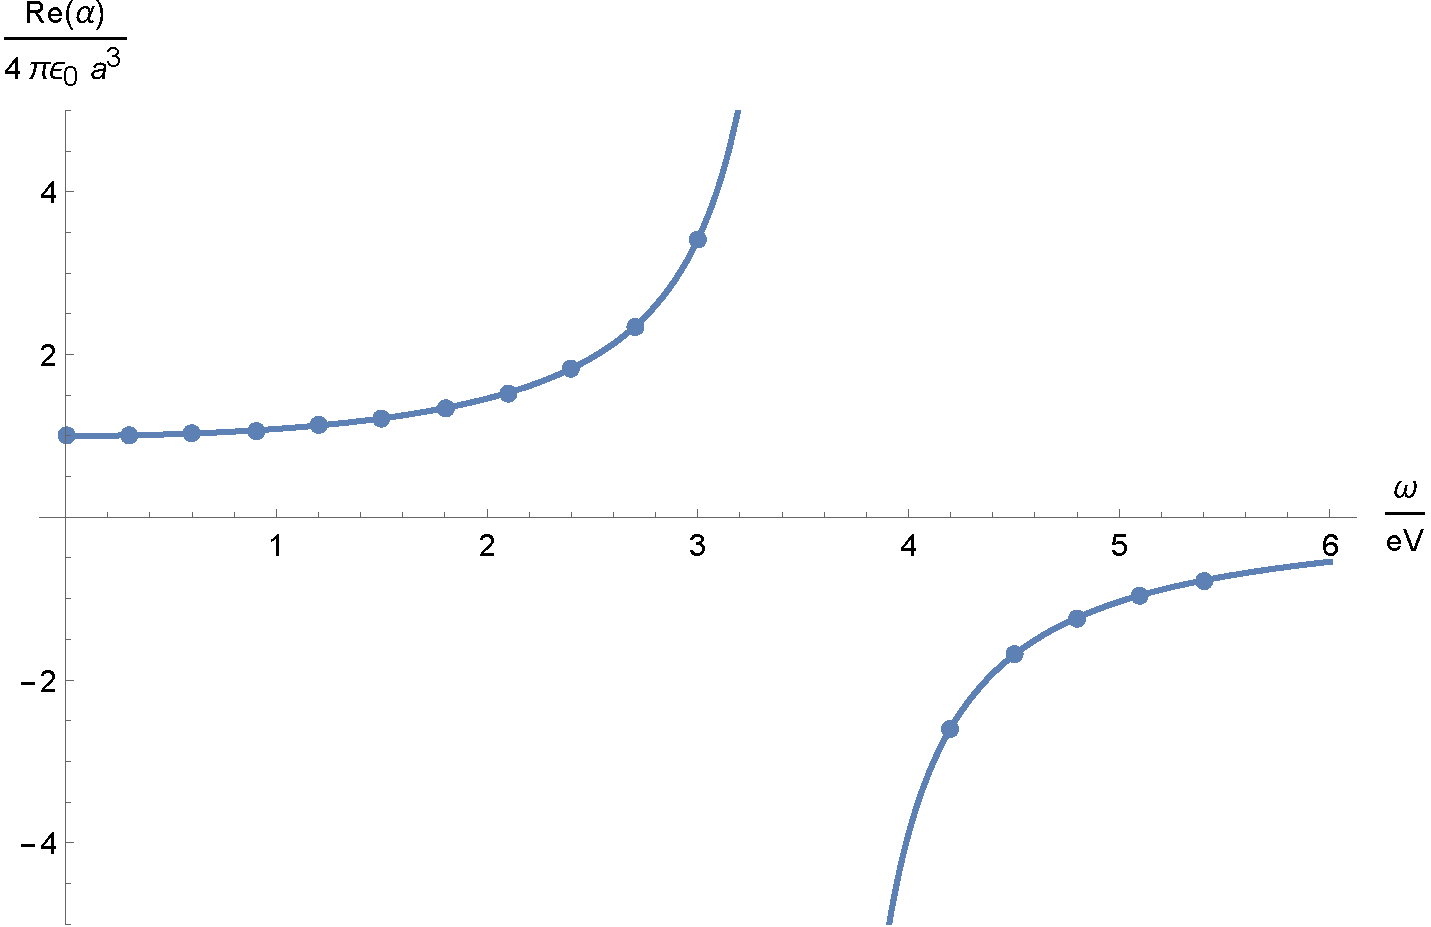
\includegraphics[width=\textwidth]{alpha-re.pdf}
    \end{subfigure}
    \begin{subfigure}{0.45\textwidth}
        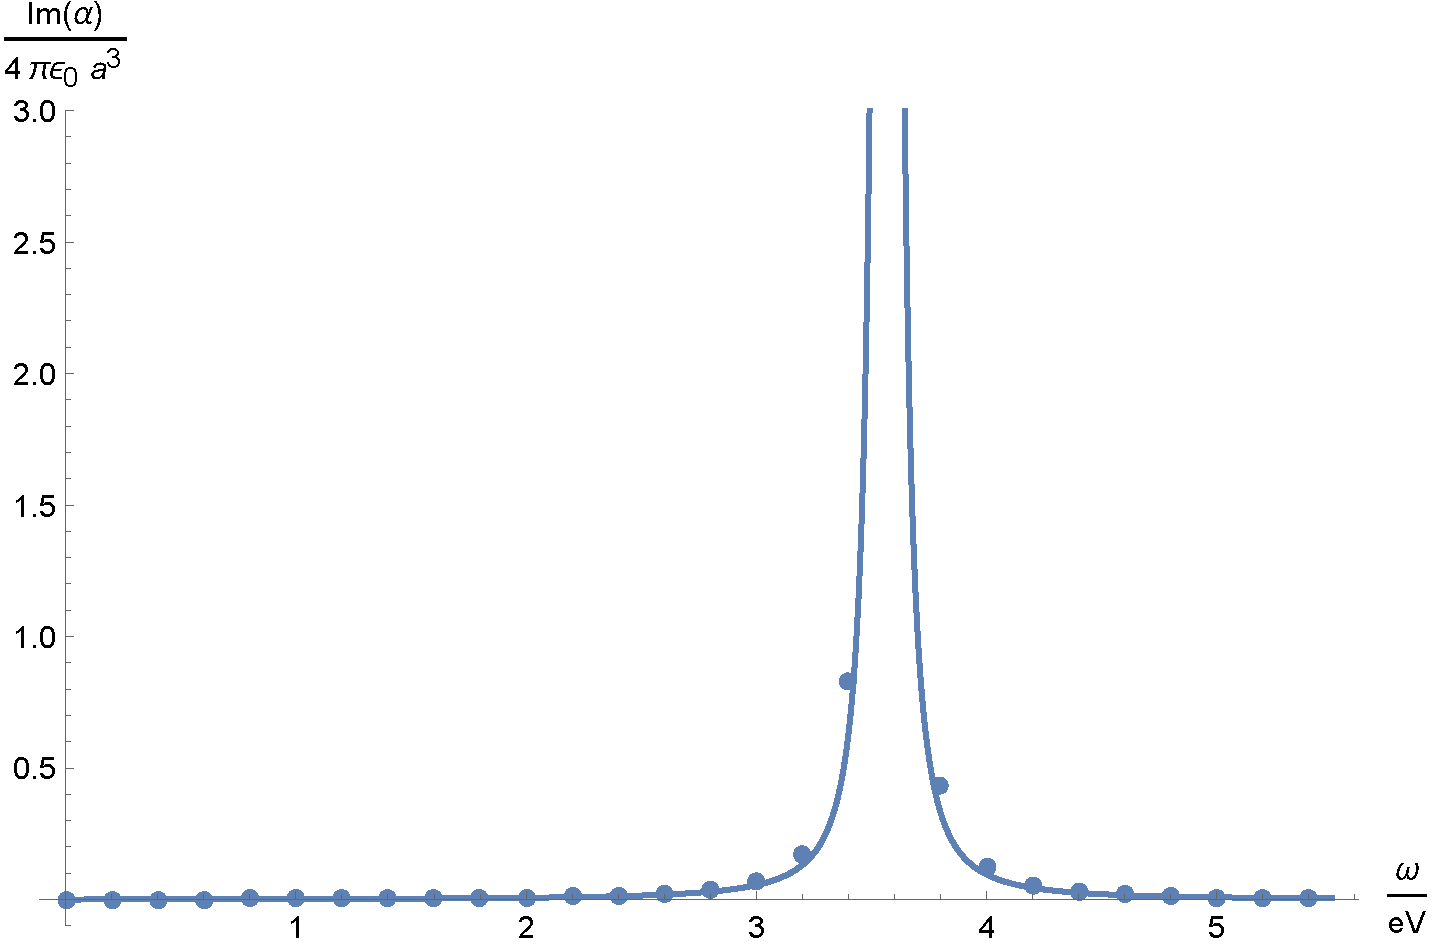
\includegraphics[width=\textwidth]{alpha-im.pdf}
    \end{subfigure}
    \caption{The real and the imaginary part of $\alpha(\omega)$. The lines are plotted by definition, and the scattered points are obtained by K-K relations. (a) The real part. (b) The imaginary part.}
    \label{fig:plot}
\end{figure}

\paragraph{Problem 1} Consider a one dimensional infinite chain on the $z$ direction consisting of metallic balls, 
each of which have radius $a$ and is made of a metal with permittivity
\begin{equation}
    \epsilon_\text{r} = 1 - \frac{\omega_\text{p}^2}{\omega (\omega + \ii \gamma)}.
\end{equation} 
When $a \to 0$, we have
\begin{equation}
    \alpha(\omega) = 4 \pi \epsilon_0 a^3 \frac{\epsilon_\text{r}(\omega) - 1}{\epsilon_\text{r}(\omega) + 2},
\end{equation}
We use Mathematica to plot the real and the imaginary part of $\alpha(\omega)$ in \prettyref{fig:plot}. 
TODO: features

\paragraph{}

\paragraph{Problem 2} We need to solve 
\begin{equation}
    \vb*{p}_m = \alpha (\vb*{E}_\text{ext}(\vb*{r}_m) + \omega^2 \mu_0 \sum_{n \neq m} \tensor{\vb*{G}}(\vb*{r}_m - \vb*{r}_n) \cdot \vb*{p}_n),
    \label{eq:p-ext}
\end{equation}
and when there is no external field, by the Bloch condition 
\begin{equation}
    \vb*{p}_m = \vb*{u} \ee^{\ii k z_m},
\end{equation}
we have 
\[
    \vb*{u} \ee^{\ii k z_m} = \alpha \omega^2 \mu_0 \sum_{n \neq m} \tensor{\vb*{G}}(\vb*{r}_m - \vb*{r}_n) \cdot \vb*{u} \ee^{\ii k z_n},
\]
\[
    \left( \tensor{\vb*{I}} - \alpha \omega^2 \mu_0 \sum_{n \neq m} \tensor{\vb*{G}}(\vb*{r}_m - \vb*{r}_n) \ee^{\ii k z_n} \ee^{- \ii k z_m}  \right) \vb*{u}  = 0,
\]
and we have 
\begin{equation}
    \tensor{\vb*{M}} = \alpha^{-1} \tensor{ \vb*{I}} - \omega^2 \mu_0 \sum_{n \neq m} \tensor{\vb*{G}}(\vb*{r}_m - \vb*{r}_n) \ee^{\ii k (z_n - z_m)}, \quad \tensor{\vb*{M}} \vb*{u} = 0,
    \label{eq:eigen-problem}
\end{equation}
and we need to evaluate 
\begin{equation}
    \tensor{\vb*{W}} = \omega^2 \mu_0 \sum_{n \neq m} \tensor{\vb*{G}}(\vb*{r}_m - \vb*{r}_n) \ee^{\ii k (z_n - z_m)}.
    \label{eq:def-w}
\end{equation}

The dyadic Green function is 
\begin{equation}
    \tensor{G}(\vb*{R}) = \frac{k_0}{4\pi} \frac{\ee^{\ii k_0 R}}{k_0 R} \Biggl( \tensor{I} \left( 1 - \frac{4\pi R}{3k_0^2} \delta(\vb*{R}) - \frac{1}{k_0^2 R^2} + \frac{\ii}{k_0 R} \right) 
        + \frac{\vb*{R} \vb*{R}}{R^2} \left( \frac{3}{k_0^2 R^2} - 1 - \frac{3\ii}{k_0 R} \right) \Biggr).
\end{equation}
Since $\vb*{R} = \vb*{r}_m - \vb*{r}_n \neq 0$, the $\delta$-function term vanishes. Since $\vb*{r}_m - \vb*{r}_n$
is along the $z$ axis, We have 
\[
    \frac{\vb*{R} \vb*{R}}{R^2} = \vb*{e}_z \vb*{e}_z, \quad R = \abs*{z_m - z_n}.
\]
Therefore, by the definition \eqref{eq:def-w}, we have 
\[
    \begin{aligned}
        \tensor{\vb*{W}} &= \omega^2 \mu_0 \sum_{m \neq n} \ee^{\ii k(z_n - z_m)} \frac{k_0}{4\pi} \ee^{\ii k_0 R}
        \Biggl( \tensor{\vb*{I}} \left( \frac{1}{k_0 R} + \frac{\ii}{k_0^2 R^2} - \frac{1}{k_0^3 R^3} \right) \\
        &\quad \quad + \vb*{e}_z \vb*{e}_z \left( - \frac{1}{k_0 R} - \frac{3 \ii}{k_0^2 R^2} + \frac{3}{k_0^3 R^3} \right) \Biggr) \\
        &= \omega^2 \mu_0 \frac{k_0}{4\pi} \left( \sum_{z_m < z_n} + \sum_{z_m > z_n} \right) \ee^{\ii k_0 R - \ii k (z_m - z_n)} \Biggl( \tensor{\vb*{I}} \left( \frac{1}{k_0 R} + \frac{\ii}{k_0^2 R^2} - \frac{1}{k_0^3 R^3} \right) \\
        &\quad \quad + \vb*{e}_z \vb*{e}_z \left( - \frac{1}{k_0 R} - \frac{3 \ii}{k_0^2 R^2} + \frac{3}{k_0^3 R^3} \right) \Biggr) \\ 
        &= \omega^2 \mu_0 \frac{k_0}{4\pi} \left( \sum_{l=1}^\infty \ee^{\ii (k_0 - k) \Lambda l} + \sum_{l=1}^\infty \ee^{\ii (k_0 + k) \Lambda l} \right) \Biggl( \tensor{\vb*{I}} \left( \frac{1}{k_0 \Lambda l} + \frac{\ii}{k_0^2 \Lambda^2 l^2} - \frac{1}{k_0^3 \Lambda^3 l^3} \right) \\
        &\quad \quad + \vb*{e}_z \vb*{e}_z \left( - \frac{1}{k_0 \Lambda l} - \frac{3 \ii}{k_0^2 \Lambda^2 l^2} + \frac{3}{k_0^3 \Lambda^3 l^3} \right) \Biggr) .
    \end{aligned}
\] 
Using formulae from \href{https://en.wikipedia.org/wiki/Polylogarithm}{Wikipedia}, we have 
\[
    \left( \sum_{l=1}^\infty \ee^{\ii (k_0 - k) \Lambda l} + \sum_{l=1}^\infty \ee^{\ii (k_0 + k) \Lambda l} \right) \frac{1}{l^s} = \li_s(\ee^{\ii (k_0 - k) \Lambda}) + \li_s(\ee^{\ii (k_0 + k) \Lambda}),
\]
So finally we have 
\begin{equation}
    \begin{aligned}
        \tensor{\vb*{W}} &= \frac{\omega^2 \mu_0 k_0}{4 \pi} \biggl(
        \frac{1}{k_0 \Lambda} (\tensor{\vb*{I}} - \vb*{e}_e \vb*{e}_z) (\li_1(\ee^{\ii (k_0 - k) \Lambda}) + \li_1(\ee^{\ii (k_0 + k) \Lambda})) \\
        &\quad \quad + \frac{\ii}{k_0^2 \Lambda^2} (\tensor{\vb*{I}} - 3 \vb*{e}_z \vb*{e}_z) (\li_2(\ee^{\ii (k_0 - k) \Lambda}) + \li_2(\ee^{\ii (k_0 + k) \Lambda})) \\
        &\quad \quad - \frac{1}{k_0^3 \Lambda^3} (\tensor{\vb*{I}} - 3 \vb*{e}_z \vb*{e}_z) (\li_3(\ee^{\ii (k_0 - k) \Lambda}) + \li_3(\ee^{\ii (k_0 + k) \Lambda})).
        \biggr)
    \end{aligned}
    \label{eq:w-explicit}
\end{equation}

\paragraph{Problem 3} When the system is in a single mode, we have $\vb*{p}_m = \alpha_\text{eff} 
\vb*{E}_\text{eig}$, and from \eqref{eq:p-ext} we have 
\[
    \alpha^{-1} \vb*{p}_m = \alpha_\text{eig}^{-1} \vb*{p}_m + \omega^2 \mu_0 \sum_{n \neq m} \tensor{\vb*{G}}(\vb*{r}_m - \vb*{r}_n) \cdot \vb*{p}_n,
\]
and we find it is equivalent to 
\begin{equation}
    \tensor{\vb*{M}} \cdot \ \vb*{u} = \frac{1}{\alpha_\text{eff}} \vb*{u} = \lambda \vb*{u}.
    \label{eq:external-eigen}
\end{equation}
The eigenvalues are inverse effective polarizabilities. \eqref{eq:external-eigen} is equivalent to 
\[
    \alpha^{-1} \vb*{u} - \tensor{\vb*{W}} \cdot \ \vb*{u} = \alpha_\text{eig}^{-1} \vb*{u},
\]
and we known that $\tensor{\vb*{W}}$ is diagonal in the $\vb*{e}_x, \vb*{e}_y, \vb*{e}_z$ basis, so the
eigenvectors are just $\vb*{e}_x, \vb*{e}_y, \vb*{e}_z$, and it is straightforward to find that the 
polarizabilities on the $x$ and $y$ directions are the same: 
\begin{equation}
    \begin{aligned}
        \alpha_\text{eig,$xy$}^{-1} &= \alpha^{-1} - \frac{\omega^2 \mu_0 k_0}{4 \pi} \biggl( \frac{1}{k_0 \Lambda} (\li_1(\ee^{\ii (k_0 - k) \Lambda}) + \li_1(\ee^{\ii (k_0 + k) \Lambda})) \\
        &\quad \quad + \frac{\ii}{k_0^2 \Lambda^2} (\li_2(\ee^{\ii (k_0 - k) \Lambda}) + \li_2(\ee^{\ii (k_0 + k) \Lambda})) - \frac{1}{k_0^3 \Lambda^3} (\li_3(\ee^{\ii (k_0 - k) \Lambda}) + \li_3(\ee^{\ii (k_0 + k) \Lambda})) \biggr),
    \end{aligned}
\end{equation}
and the polarizability on the $z$ direction is 
\begin{equation}
    \begin{aligned}
        \alpha_\text{eig,$z$}^{-1} &= \alpha^{-1} - \frac{\omega^2 \mu_0 k_0}{4 \pi} \biggl( - \frac{2\ii}{k_0^2 \Lambda^2} (\li_2(\ee^{\ii (k_0 - k) \Lambda}) + \li_2(\ee^{\ii (k_0 + k) \Lambda})) \\
        &\quad \quad  + \frac{2}{k_0^3 \Lambda^3} (\li_3(\ee^{\ii (k_0 - k) \Lambda}) + \li_3(\ee^{\ii (k_0 + k) \Lambda})) \biggr).
    \end{aligned}
\end{equation}

\paragraph{Problem 4} In the $c \to \infty$ limit, $k_0 \to 0$, so all $1 / (k_0 \Lambda)^s$ terms in \eqref{eq:w-explicit} diverges,
and only the most divergent terms where $s=3$ are important, i.e. we only keep the near field terms 
in $\tensor{\vb*{G}}$, and we have 
\[
    \tensor{\vb*{W}} = \omega^2 \frac{\mu_0 k_0}{4 \pi} \left( \frac{3 \vb*{e}_z \vb*{e}_z - \tensor{\vb*{I}}}{k_0^3 \Lambda^3} \right) (\li_3(\ee^{\ii k \Lambda}) + \li_3 (\ee^{- \ii k \Lambda})).
\] 
In the $\gamma \to 0$ limit, we have 
\[
    \frac{1}{\alpha} = \frac{1}{4 \pi \epsilon_0 a^3} \frac{\epsilon_\text{r} + 2}{\epsilon_\text{r} - 1}
    = \frac{1}{4 \pi \epsilon_0 a^3} \frac{\omega_\text{p}^2 - 3 \omega^2}{\omega_\text{p}^2}. 
\]
So we have 
\[
    \frac{1}{\alpha} = \frac{1}{4 \pi \epsilon_0 a^3} \frac{\omega_\text{p}^2 - 3 \omega^2}{\omega_\text{p}^2} \vb*{u} = \underbrace{\omega^2 \frac{\mu_0 }{4 \pi} \frac{1}{k_0^2}}_{= \frac{\mu_0 c^2}{4\pi} = \frac{1}{4 \pi \epsilon_0}} \left( \frac{3 \vb*{e}_z \vb*{e}_z - \tensor{\vb*{I}}}{ \Lambda^3} \right) (\li_3(\ee^{\ii k \Lambda}) + \li_3 (\ee^{- \ii k \Lambda})) \vb*{u},
\]
and finally \eqref{eq:eigen-problem} can be written as 
\begin{equation}
    \tensor{\vb*{H}} \cdot \ \vb*{u} = \frac{\omega^2}{\omega_\text{p}^2} \vb*{u},
\end{equation}
where 
\begin{equation}
    \tensor{\vb*{H}} = \frac{1}{3} \left(1 - \frac{a^3}{\Lambda^3} (3 \vb*{e}_z \vb*{e}_z - \tensor{\vb*{I}}) \right) (\li_3(\ee^{\ii k \Lambda}) + \li_3 (\ee^{- \ii k \Lambda}))
    \label{eq:eff-ham}
\end{equation}
By definition we know that $(\li_3(\ee^{\ii k \Lambda}) + \li_3 (\ee^{- \ii k \Lambda}))$ is a real number, so 
\eqref{eq:eff-ham} is a Hermitian matrix, and therefore qualifies as a Hamiltonian. Again, we find that 
$\tensor{\vb*{H}}$'s eigenvectors are $\vb*{e}_x$, $\vb*{e}_y$ and $\vb*{e}_z$, and the eigenvalues are 
\begin{equation}
    \frac{\omega_{xy}^2}{\omega_\text{p}^2} = \frac{1}{3} \left( 1 + \frac{a^3}{\Lambda^3} \right) (\li_3(\ee^{\ii k \Lambda}) + \li_3 (\ee^{- \ii k \Lambda})),
\end{equation}
and 
\begin{equation}
    \frac{\omega_{z}^2}{\omega_\text{p}^2} = \frac{1}{3} \left( 1 - \frac{2a^3}{\Lambda^3} \right) (\li_3(\ee^{\ii k \Lambda}) + \li_3 (\ee^{- \ii k \Lambda})).
\end{equation}

\end{document}